\documentclass[12pt]{beamer}

\usepackage{amsthm}
\usepackage[all]{xy}
\usepackage{graphicx}
\usepackage{listings}
\usepackage{hyperref}
\usepackage[shorthands=off,slovak]{babel}
\usepackage[utf8]{inputenc}
\usepackage[T1]{fontenc}


\mode<presentation>
{\usetheme{Madrid}
\usecolortheme{beaver}}

\title[Prezentácia o pythone]{Python (Proseminár z \TeX u)}
\author[A. Matejov]{Adrián Matejov}

\institute{FMFI UK v Bratislave}

\addtobeamertemplate{background canvas}{\transwipe}{}

\begin{document}

\begin{frame}
    \titlepage
\end{frame}

\begin{frame}{Obsah}
    \tableofcontents
\end{frame}

\begin{frame}{XYMatrix obrázok na začiatok}
$$ \xymatrix@=0.3cm@1{
    & & & & & *++[Fo]{}\ar@{-}[ddrrrrrrr] \ar@{-}[dddrrrrr] \ar@{-}[dddddll] \ar@{-}[ddddddlllll] & & & & & & & & & \\
    \\
    & & & & & & & & & & & & *++[Fo]{} \ar@{-}[dll] \ar@{-}[ddddddrr] \ar@{-}[ddddlll]|!{[dll];[ddddddddr]}\hole & & \\
    & & & & & & & & & & *++[Fo]{} \ar@{-}[dddddddrrr] \ar@{-}[ddddddlllll] & & & & \\
    \\
    & & & *++[Fo]{} \ar@{-}[dlll] \ar@{-}[drrrrrr]|!{[uurrrrrrr];[ddddrr]}\hole \ar@{-}[dddddrrr]|!{[uurrrrrrr];[ddddrr]}\hole|!{[ddddrr];[dddddrrrrrrrrrr]}\hole & & & & & & & & & & & \\
    *++[Fo]{} \ar@{-}[dddrrrrr] \ar@{-}[dddddddrr] & & & & & & & & & *++[Fo]{} \ar@{-}[ddrrrrr]|!{[uuur];[ddddrrrr]}\hole \ar@{-}[ddddlll]|!{[dddllll];[ddddrrrr]}\hole & & & & & \\
    \\
    & & & & & & & & & & & & & & *++[Fo]{} \ar@{-}[ddl] \ar@{-}[ddddddllll]|!{[uuuuullll];[ddl]}\hole|!{[dlllllllll];[ddl]}\hole \\
    & & & & & *++[Fo]{} \ar@{-}[drrrrrrrr] \ar@{-}[ddddlll] & & & & & & & & & \\
    & & & & & & *++[Fo]{} \ar@{-}[dddllll] \ar@{-}[ddddrrrr] & & & & & & & *++[Fo]{} \ar@{-}[ddddlll] & \\
    \\
    \\
    & & *++[Fo]{} \ar@{-}[drrrrrrrr] & & & & & & & & & & & & \\
    & & & & & & & & & & *++[Fo]{} & & & & \\} $$
\end{frame}

\section{Úvod}
\begin{frame}{Úvod - čo je to Python?}
    \begin{center}
Python je interpretovaný, interaktívny programovací jazyk, ktorý vytvoril
Guido van Rossum, pôvodne ako skriptovací jazyk pre Amoeba OS schopný
systémových volaní. Python je často porovnávaný s jazykmi Tcl, Perl, Scheme,
Java a Ruby. Python je vyvíjaný ako open source projekt, a je v súčasnosti
pri verzii 3.4.2
    \end{center}
\end{frame}

\section{Motivácia}
\begin{frame}{Motivácia (Hello world)}
    \begin{figure}
        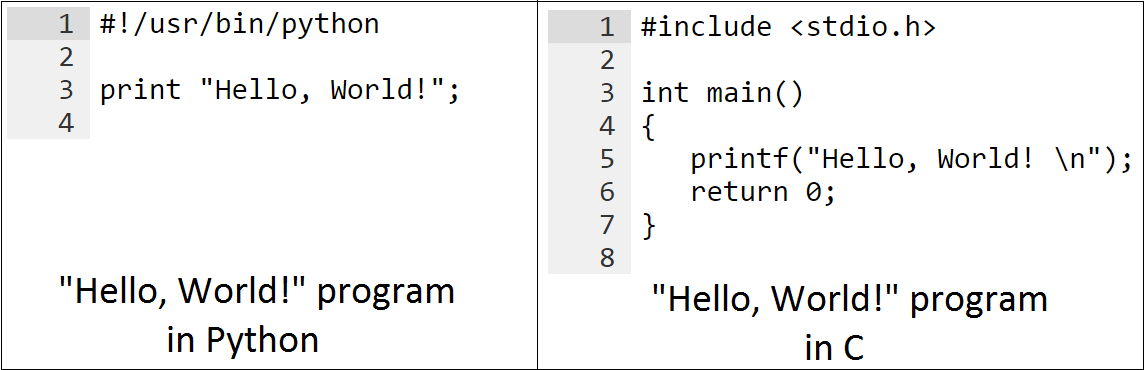
\includegraphics[width=0.8\textwidth]{helloworld.png}
        \caption{Rozdiel medzi hello world v Pythone a C}
        \label{fig1}
    \end{figure}
\end{frame}

\section{Dátové typy}
\begin{frame}{Dátové typy}
    \begin{itemize}
    \item celé čísla

    \uncover<2->{\item čísla s pohyblivou desatinnou čiarkou}

    \uncover<3->{\item celé čísla neobmedzenej dĺžky}

    \uncover<4->{\item komplexné čísla}

    \end{itemize}
\end{frame}

\begin{frame}{Odsadzovanie blokov kódu}
    \only<1>{V jazykoch, ktoré používajú blokovú štruktúru zdedenú po ALGOLe (vrátane Pascalu, C, Perlu a mnohých iných) bloky kódu sú oddelené pomocou zátvoriek alebo kľúčových slov ako begin a end v Pascale. Avšak vo všetkých týchto jazykoch programátori obyčajne používajú odsadzovanie kódu v bloku od kraja, aby vizuálne oddelili blok od ostatného kódu. \newline \newline
Python na rozdiel od toho požičiava vlastnosť z málo známeho jazyka ABC - namiesto interpunkcie alebo kľúčových slov používa samotné odsadzovanie na určenie bloku.}

    \only<2>{\begin{figure}
        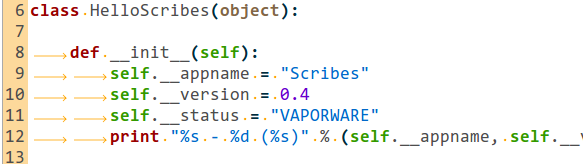
\includegraphics[width=0.8\textwidth]{indentation.png}
        \caption{Ukážka odsadzovania kódu v pythone}
        \label{fig2}
    \end{figure}}
\end{frame}

\section{Zhrnutie Python3 builtin types}
\begin{frame}{Python3 builtin types}
    \begin{center}
    \begin{tabular}{|c|l|l|}
        \hline
        \textbf{Typ} & \textbf{Popis} & \textbf{Príklad} \\ \hline
        \uncover<2->{\texttt{str}} & \uncover<3->{String, sekvencia znakov} & \uncover<4->{\texttt{'Python',"Python"}}\\ \hline
        \uncover<2->{\texttt{bytearray}} & \uncover<3->{Sekvencia bytov} & \uncover<4->{\texttt{bytearray(b'A')}} \\ \hline
        \uncover<2->{\texttt{bytes}} & \uncover<3->{Sekvencia bytov} & \uncover<4->{\texttt{b'ASCII'}} \\ \hline
        \uncover<5->{\texttt{list}} & \uncover<6->{Obsahuje mix. typy} & \uncover<7->{\texttt{[4.0,"Str",True]}}\\ \hline
        \uncover<5->{\texttt{tuple}} & \uncover<6->{Ako list, ale immutable} & \uncover<7->{\texttt{(4.0,"Str",True)}} \\ \hline
        \uncover<5->{\texttt{set}} & \uncover<6->{Množina, mutable} & \uncover<7->{\texttt{\string{4.0,"Str",True\string}}} \\ \hline
    \end{tabular}
    \end{center}
\end{frame}

\begin{frame}{Python3 builtin types 2}
    \begin{center}
    \begin{tabular}{|c|l|l|}
        \hline
        \textbf{Typ} & \textbf{Popis} & \textbf{Príklad} \\ \hline
        \uncover<2->{\texttt{frozenset}} & \uncover<3->{Množina, immutable} & \uncover<4->{\texttt{frozenset([4.0,True])}} \\ \hline
        \uncover<2->{\texttt{dict}} & \uncover<3->{Asoc. pole, kľúč:hodnota} & \uncover<4->{\texttt{\string{"kluc": False\string}}} \\ \hline
        \uncover<2->{\texttt{int}} & \uncover<3->{Integer, neobmedz. rozsah} & \uncover<4->{\texttt{42}} \\ \hline
        \uncover<5->{\texttt{float}} & \uncover<6->{Reálne číslo} & \uncover<7->{\texttt{42.1548}} \\ \hline
        \uncover<5->{\texttt{complex}} & \uncover<6->{Komplexné číslo} & \uncover<7->{\texttt{3+7j}}\\ \hline
        \uncover<5->{\texttt{bool}} & \uncover<6->{Boolean hodnota} & \uncover<7->{\texttt{True, False}} \\ \hline
    \end{tabular}
    \end{center}
\end{frame}

\section{Matika v Pythone}
\begin{frame}{Matika v pythone}
    \setbeamercovered{transparent}
    \begin{itemize}
        \item<1>Štandardné matematické operácie +, -, *, /
        \item<2>Špecialita na umocňovanie \texttt{5**3} ($5^{3}$)
        \item<3> Python $<=$ 2.1 používa delenie ako v C. Keď sú oba operandy celé čísla,
                tak sa použije celočíselné delenie, inak delenie reálnych čísel.
            Celočíselné delenie zaokrúhluje sa smerom k 0.
        \item<4> Od pythonu 2.2 máme operátor \texttt{//},
                ktorý predstavuje celočíselné delenie ($7.5 // 3 = 2.0$).
                Zaokrúhľuje smerom k $-\infty$
        \item<5> Ohraničenie zdola aj zhora (\texttt{a < x < b}) - vráti True/False
            podľa toho či číslo patrí do intervalu $(a, b)$
    \end{itemize}
\end{frame}

\section{Lambda výrazy}
\begin{frame}{Lambda výrazy}
    Pomocou kľúčového slova lambda môžeme vytvárať malé anonymné funkcie.
    Bloky \textbf{lambda} v Pythone môžu obsahovať len jeden výraz a nemôžu obsahovať
    príkazy. Tu je funkcia, ktorá vracia súčet svojich dvoch argumentov.\\
    Príklad:
    \begin{center}
        \texttt{lambda a, b: a+b}
    \end{center}
\end{frame}

\section{Knižnice}
\begin{frame}{Knižnice PyPi}
    Python má veľkú základňu tzv. standard libraries, ktoré sú jeho veľkou
    zbraňou. Implementujú totiž veľmi veľa užitočných nástrojov pre budovanie
    vašej aplikácie.\\
    Dajú sa taktiež, ako v iných jazykoch, importovať balíčky, 
    ktoré sú po vačšinou umiestnené na serveri
    \href{https://pypi.python.org/pypi}{pypi (https://pypi.python.org/pypi)} \\
    Inštalujú sa cez príkazový riadok nasledujúcim príkazom \\
    \begin{center}
        \texttt{\$ pip install nazovbalicka}
    \end{center}
\end{frame}

\section{Command line interpreter}
\begin{frame}{Command line interpreter}
    Interpreter Pythonu tiež podporuje interaktívny režim, v ktorom výrazy
    môžu byť zadávané z terminálu a môžeme okamžite vidieť výsledok. Je to
    výhoda pre tých, ktorí sa učia jazyk, ale aj pre skúsených vývojárov: časti
    kódu môžu byť testované v interaktívnom režime pred tým, ako budú
    integrované do programu

    \begin{figure}
        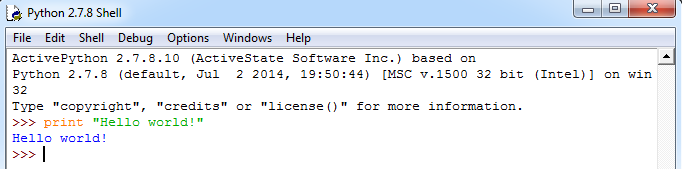
\includegraphics[width=0.8\textwidth]{idle.png}
        \caption{Python interpreter}
        \label{fig3}
    \end{figure}
\end{frame}

\section{Literatúra}
\begin{frame}{Literatúra}
    \begin{itemize}
        \item Wiki \url{https://sk.wikipedia.org/wiki/Python_(programovac\%C3\%AD_jazyk)}
        \item EN Wiki \url{https://en.wikipedia.org/wiki/Python_(programming_language)}
    \end{itemize}
\end{frame}

\begin{frame}
    \begin{center}
        \textbf{Ďakujem za pozornosť}
    \end{center}
\end{frame}
\end{document}
